%% ============================================================================
\section{Signal Processing and Feature Extraction}
\label{sec:pipeline}
%% ============================================================================
This section converts the acquired segments into the feature sets used for regression: the signals are first inspected qualitatively, then decomposed into frequency sub-bands, and finally summarised by a set of time- and frequency-domain features per band.

\subsection{Waveforms and spectrograms}

Fig.~\ref{fig:waveforms} shows the waveforms of four segments for both the AE and US channels, and Fig.~\ref{fig:spectrograms} shows the spectrograms of all segments over time. AE and US qualitatively display clearly different waveforms and frequency content in all segments. AE in general contains spectral energy from \SI{50}{kHz} to \SI{1}{MHz} as expected from the AE sensor and band-pass filter applied during data acquisition. Some energy also appears above 1 MHz, but as its origin could not be reliably established it is excluded from subsequent analysis. \todo{Change this depending on the data, the noise from the oscilloscope, and the final conclustion about speed reconstruction.} US shows highest energy concentration in the spectral band from \SI{0}{kHz} to \SI{20}{kHz}, consistent with heterodyning, but also displays energy from \SI{20}{kHz} to \SI{100}{kHz}. This is attributed to heterodyning artifacts consisting of sums and multiples of the carrier and original frequencies.

\begin{figure}[H]
\centering
\includegraphics[width=1\textwidth]{figures/eda_waveforms.png}
\caption{Waveforms of AE and US signals from the same segments for different values of $\kappa$. AE shows transient energy bursts consistent with impulsive contact-related events. US shows a more regular, lower frequency, non-stationary waveform.}
\label{fig:waveforms}
\end{figure}\todo{Select new files. The first file shows weird waveforms for both AE and US (clipping). Maybe same y-axis? Cut off at 1MHz and write oscilloscope noise reason.}

\begin{figure}[H]
\centering
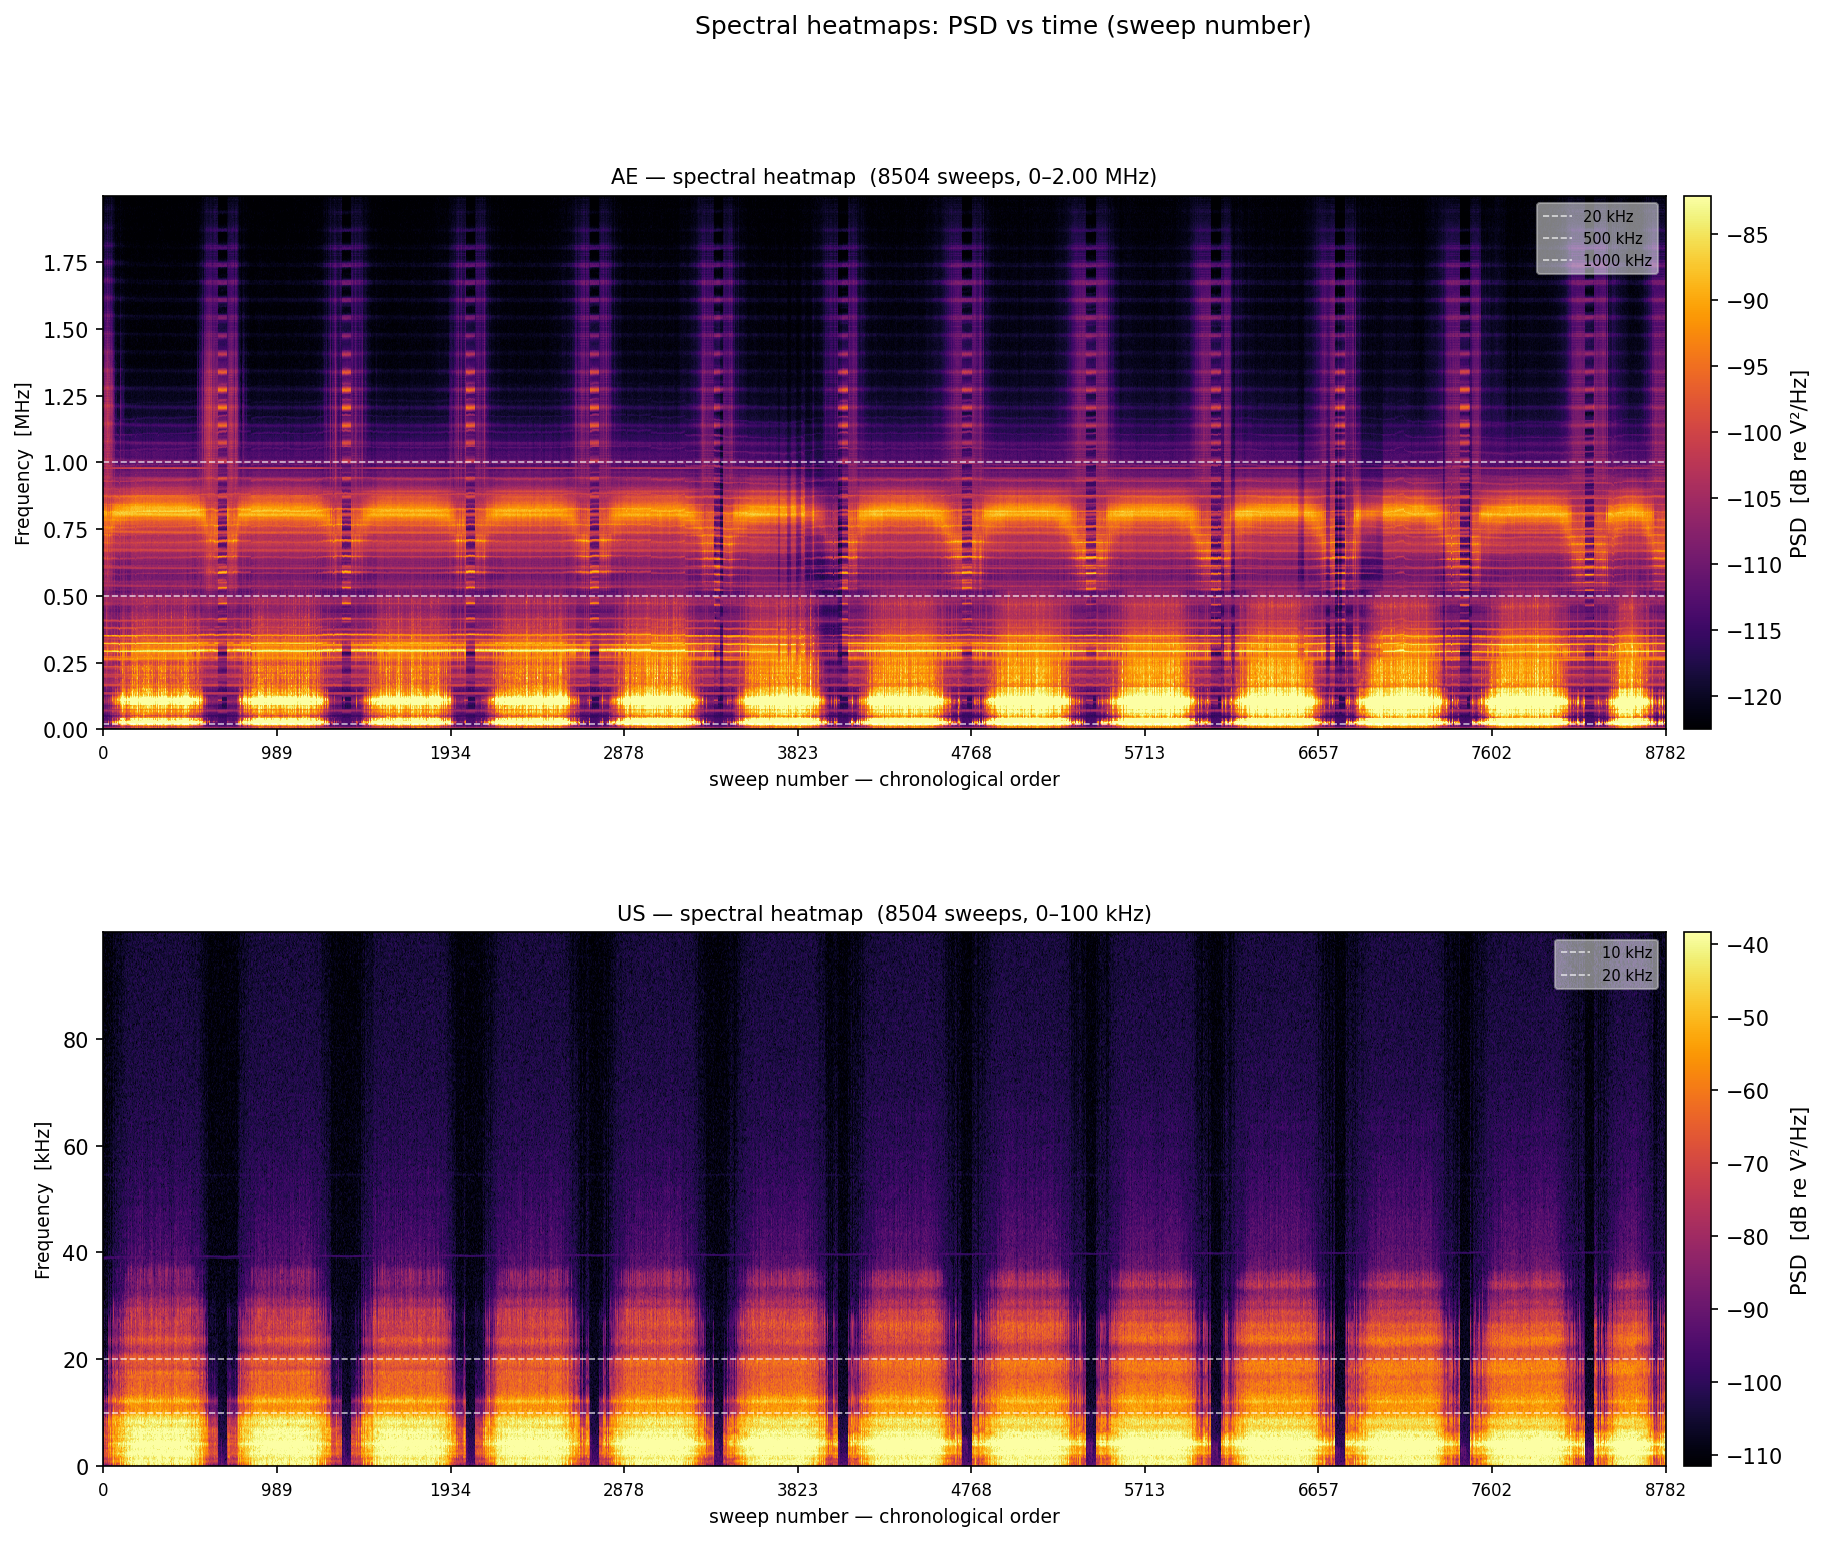
\includegraphics[width=0.8\textwidth]{figures/eda_spectrogram_chronological.png}
\caption{Spectrograms of the raw AE and US ordered chronologically by acquisition time. PSD is calculated with Welch's method, Hann windows, 50\% overlap, and segment lengths of 4096 samples (AE) and 65536 samples (US).}
\label{fig:spectrograms}
\end{figure}\todo{Finalize specrograms with correct colors, ranges, and dashed lines for sub-bands}

\subsection{Sub-band decomposition}
\label{subsec:filter_bands}
The AE and US signals are decomposed into frequency sub-bands prior to feature extraction, since the predictive information related to $\kappa$ is expected to be more localised in sub-bands than in broadband signals~\cite{renhart_ae_2021, zhang_coupled_2026,jakobsen_detecting_2023,zhang_graph_2024}. For the AE channel, two sub-bands are extracted in addition to the broadband signal: 20--500~kHz and 500~kHz--1~MHz, containing bands of spectral energy which upon visual inspection of Fig.~\ref{fig:spectrograms} vary with the operating conditions. Content above the \SI{1}{MHz} coupler low-pass is excluded from the feature set. The coupler additionally high-passes at \SI{50}{kHz} before digitisation (Section~\ref{subsec:rig}), so the AE broadband spans \SI{50}{kHz}--\SI{1}{MHz} and the 20--500~kHz sub-band---a nominal digital passband---carries effective content of 50--500~kHz, as no energy remains below \SI{50}{kHz}. For the US channel, the signal spans the probe's 0--100~kHz acquisition band, and three sub-bands are extracted in addition to the broadband signal: 0--10~kHz and 10--20~kHz within the nominal heterodyned baseband, and 20--100~kHz. The 0--20~kHz bands correspond to the audible heterodyned baseband commonly used in commercial passive ultrasound instruments, while 20--100~kHz evaluates whether additional ultrasonic information retained after acquisition contributes to prediction. The sub-bands are summarised in Table~\ref{tab:subbands}. The goal of sub-band feature extraction is not to find the most informative, physically motivated frequency bands, but to extract more information than from simple broadband features. Usefulness of sub-bands is expected to vary across test rig setups, bearings, lubricants, and operating conditions, so data mining for optimal sub-bands is furthermore expected to overfit on this particular setup. All decompositions use 5th-order Butterworth filters applied forward--backward giving zero phase distortion and a 10th-order effective magnitude response.

\begin{table}[htbp]
\centering
{\small\setstretch{1}%
\begin{tabular}{@{} l l l r @{}}
\toprule
\textbf{Channel} & \textbf{Sub-band} & \textbf{Filter type} & \textbf{Frequency range} \\
\midrule
AE & Broadband  & Band-pass       & 50\,kHz--1\,MHz        \\
AE & Sub-band 1 & Band-pass & 20--500\,kHz     \\
AE & Sub-band 2 & Band-pass & 500\,kHz--1\,MHz \\
US & Broadband  & Low-pass  & 0--100\,kHz      \\
US & Sub-band 1 & Band-pass & 0--10\,kHz       \\
US & Sub-band 2 & Band-pass & 10--20\,kHz      \\
US & Sub-band 3 & Band-pass & 20--100\,kHz     \\
\bottomrule
\end{tabular}}
\caption{Frequency sub-bands used for signal pre-filtering before feature extraction. AE ranges reflect the coupler's \SI{50}{kHz}--\SI{1}{MHz} passband (Section~\ref{subsec:rig}); the 20--500~kHz sub-band is the nominal digital filter, with effective content 50--500~kHz.}
\label{tab:subbands}
\end{table}

\subsection{Feature set}
\label{subsec:features_extract}

Features are computed from the voltage signal of each segment--sensor pair, for the broadband signal and for each sub-band. In total 14 features are computed, comprising 8 time-domain and 6 frequency-domain statistics, as listed in Table~\ref{tab:features}. The set is deliberately canonical: commonly used features such as standard deviation, variance, peak, impulse factor, and RMS frequency are approximately equivalent to products of the chosen features and are therefore omitted, so that no feature is a deterministic function of another. All features (without the specific sub-bands) have previously been applied to signals for bearing condition monitoring and LCM~\cite{jakobsen_detecting_2023,zhang_graph_2024}; the Hjorth parameters originate from EEG analysis~\cite{hjorth_eeg_1970}. Mobility, the ratio between the standard deviations of a signal's first time-derivative and of the signal itself, is a time-domain estimate of the signal's mean frequency: it rises as energy shifts toward higher frequencies within the band. Complexity, the mobility of the derivative relative to the mobility of the signal, measures spectral spread: it attains its minimum of one for a pure sinusoid and grows as the signal departs from a single dominant frequency toward broadband content.

\begin{table}[htbp]
\centering
{\small\setstretch{1}%
\begin{tabular}{@{} l l @{}}
\toprule
\textbf{Name} & \textbf{Formula} \\
\midrule
\multicolumn{2}{@{}l}{\itshape Time domain} \\
\addlinespace[2pt]
RMS & $\sqrt{N^{-1}\sum_{n}x_n^2}$ \\[3pt]
Skewness & $N^{-1}\sum_{n}[(x_n-\bar{x})/\sigma]^3$ \\[3pt]
Kurtosis & $N^{-1}\sum_{n}[(x_n-\bar{x})/\sigma]^4$ \\[3pt]
Crest factor & $x_{\text{peak}}/x_{\text{RMS}}$ \\[3pt]
Shape factor & $x_{\text{RMS}}\,/\,(N^{-1}\sum_n|x_n|)$ \\[3pt]
Margin factor & $x_{\text{peak}}\,/\,(N^{-1}\sum_n\sqrt{|x_n|})^2$ \\[3pt]
Hjorth mobility & $M(x) = [\operatorname{Var}(x')/\operatorname{Var}(x)]^{1/2}$ \\[3pt]
Hjorth complexity & $M(x')/M(x)$ \\
\midrule
\multicolumn{2}{@{}l}{\itshape Frequency domain} \\
\addlinespace[2pt]
Dominant frequency & $f_{\arg\max_k S_k^2}$ \\[3pt]
Centre frequency & $f_c = \sum_k f_k S_k\,/\,\Sigma S$ \\[3pt]
Spectral bandwidth & $\sigma_w = \big(\sum_k(f_k-f_c)^2 S_k\,/\,\Sigma S\big)^{1/2}$ \\[3pt]
Spectral skewness & $\sum_k(f_k-f_c)^3 S_k\,/\,(\sigma_w^3\,\Sigma S)$ \\[3pt]
Spectral kurtosis & $\sum_k(f_k-f_c)^4 S_k\,/\,(\sigma_w^4\,\Sigma S)$ \\[3pt]
Spectral flatness & $\exp(K'^{-1}\!\sum_{k:S_k>0}\!\ln S_k)\,/\,\bar{S}$ \\
\bottomrule
\end{tabular}}
\caption{The 14 extracted features: 8 time-domain and 6 frequency-domain.  Notation: $N$ signal length; $n, k = 1,\ldots,N$; $\bar{x}$ sample mean; $\sigma$ population standard deviation; $x_{\text{peak}} = (\max x - \min x)/2$ half the peak-to-peak range; $x'$ the first time-derivative of the signal; $S_k = |X_k|$ one-sided FFT magnitude at bin~$k$; $f_k$ the corresponding frequency; $\bar{S}$ arithmetic mean of $\{S_k\}$; $\Sigma S = \sum_k S_k$; $K'$ the number of bins with $S_k > 0$.}
\label{tab:features}
\end{table}

All frequency-domain features are computed from the one-sided FFT magnitude spectrum of the segment. The spectral skewness and kurtosis are standardised by
$\sigma_w^p\,\Sigma S$ and are therefore dimensionless and invariant to overall signal amplitude, so that spectral-shape information is separated from the amplitude
information carried by RMS.

Extracting the 14-feature set independently for the broadband signal and each sub-band yields \resNcandAe~AE features (broadband plus two sub-bands) and \resNcandUs~US features (broadband plus three sub-bands) per segment. Features are named by channel, band, and statistic (e.g.\ \texttt{AE\_500-1000kHz\_\_mobility});\todo{Change this once prettier names have been decided upon.} broadband features carry no band prefix. These two sets, and their union (the combined AE+US set, $\resNcandAe + \resNcandUs$ features), define the three sensor configurations---AE-only, US-only, and combined.

The extracted features are not assumed to represent lubrication-specific quantities. Instead, they provide a compact representation of acoustic signal characteristics that may contain contributions from lubrication-dependent contact dynamics, operating conditions, structural transmission effects, and sensor coupling. The subsequent analysis therefore examines what the features respond to (Section~\ref{sec:features}) and whether the two channels contribute complementary information to $\kappa$ regression (Sections~\ref{sec:modelling}--\ref{sec:results}).